
\documentclass[runningheads, a4paper, oribibl]{llncs}

\setcounter{tocdepth}{3}
\usepackage{graphicx}
\usepackage{float}
\graphicspath{{../images/}}
\usepackage{epstopdf}
\usepackage{standalone}
\usepackage{xcolor}
\usepackage{tikz}
\usetikzlibrary{fit}
\usetikzlibrary{shapes,snakes,calc}



\usepackage{listings, color}

\definecolor{dkgreen}{rgb}{0,0.6,0}
\definecolor{gray}{rgb}{0.5,0.5,0.5}
\definecolor{mauve}{rgb}{0.58,0,0.82}



\lstset{frame=tb,
  language=Matlab,
  aboveskip=3mm,
  belowskip=3mm,
  showstringspaces=false,
  columns=flexible,
  basicstyle={\small\ttfamily},
  numbers=none,
  numberstyle=\tiny\color{gray},
  keywordstyle=\color{blue},
  commentstyle=\color{dkgreen},
  stringstyle=\color{mauve},
  breaklines=true,
  breakatwhitespace=false,
  tabsize=2,
  numbers=left,
  numbersep=5pt,
  title=\lstname
}



\usepackage[section]{placeins}

\usepackage{amsmath,amssymb, cancel}
%
\usepackage{url}
\urldef{\mailsa}\path|201501005@daiict.ac.in|
\urldef{\mailsb}\path|201501422@daiict.ac.in|
\newcommand{\keywords}[1]{\par\addvspace\baselineskip
\noindent\keywordname\enspace\ignorespaces#1}


\renewcommand\thesubsection{\thesection(\alph{subsection})}


\begin{document}

\mainmatter

\title{High Performance Computing Report}

\titlerunning{High Performance Computing Report}

\author{Amarnath Karthi\\Chahak Mehta}%
%
\authorrunning{Amarnath Karthi \& Chahak Mehta}
\institute{Dhirubhai Ambani Institute of Information and Communication Technology\\
  \mailsa\\
  \mailsb\\
}

\maketitle
\section{Implementation Details (Basic matrix multiplication)}
\subsection{Brief and clear description about the Serial implementation}
The serial implementation involves basic matrix multiplication using 3 nested loops.
\begin{equation}
    C_{ij} = \sum A_{ik}B_{kj}
\end{equation}
\subsection{Brief and clear description about the implementation of the approach (Parallelization Strategy, Mapping of computation to threads)}
The parallelization is achieved by load distribution of the middle loop over several processors, using the OpenMP library. We will be using the \textbf{omp parallel for directive}.
\section{Complexity and Analysis}
\subsection{Complexity of serial code}
Cubic time complexity : $O(n^3)$.
This is because of the 3 nested loops, each having an $O(n)$ runtime complexity by itself.
\subsection{Theoretical Speedup (using asymptotic analysis, etc.)}
For an n core system, the theoretical speedup is approximately n.
\newpage
\section{Curve Based Analysis}
\subsection{Time Curve related analysis (as no. of processor increases)}
\begin{figure}[h]
    \centering
    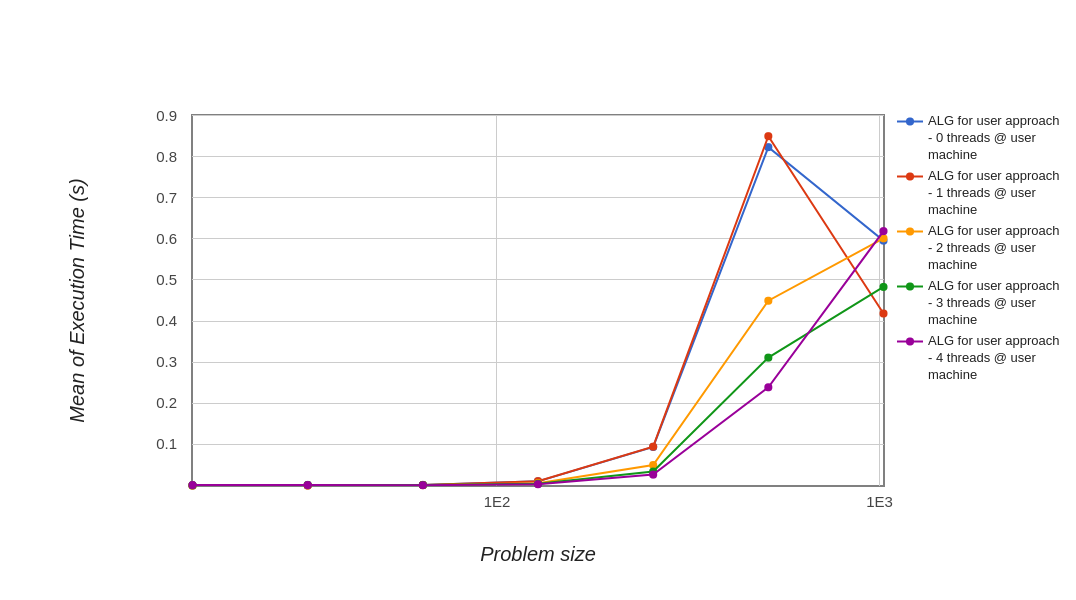
\includegraphics[width=\textwidth]{p1.png}
    \caption{Execution time for simple matrix multiplication}
    \label{fig:p1}
\end{figure}
For small problem sizes, the overhead of adding 1 extra core to the solution outweighs the advantages given by it. Thus for small input sizes, the execution time is higher for a higher number of cores. As the problem size increases, the overhead becomes insignificant in front of the compute time, which decreases drastically when a larger number of cores are used. This is quite natural because the work is shared equally amongst all processors.

\subsection{Speedup Curve related analysis (as problem size and no. of processors increase)}
The speedup is bound by "n", the number of cores. Therefore, irrespective of the problem size, the speedup is always lesser than n for n cores. For small problem sizes, the speedup is less than one if we use more cores. This again indicates that the load is too small to be parallelized efficiently. For very large problem sizes we see almost a constant speedup. This indicates that saturation has been achieved.  For 4 cores and a problem size of 512,  we get a speedup of approximately 3.2, whereas for 2 cores we get a speedup of 1.78.
\newpage
\begin{figure}[t]
    \centering
    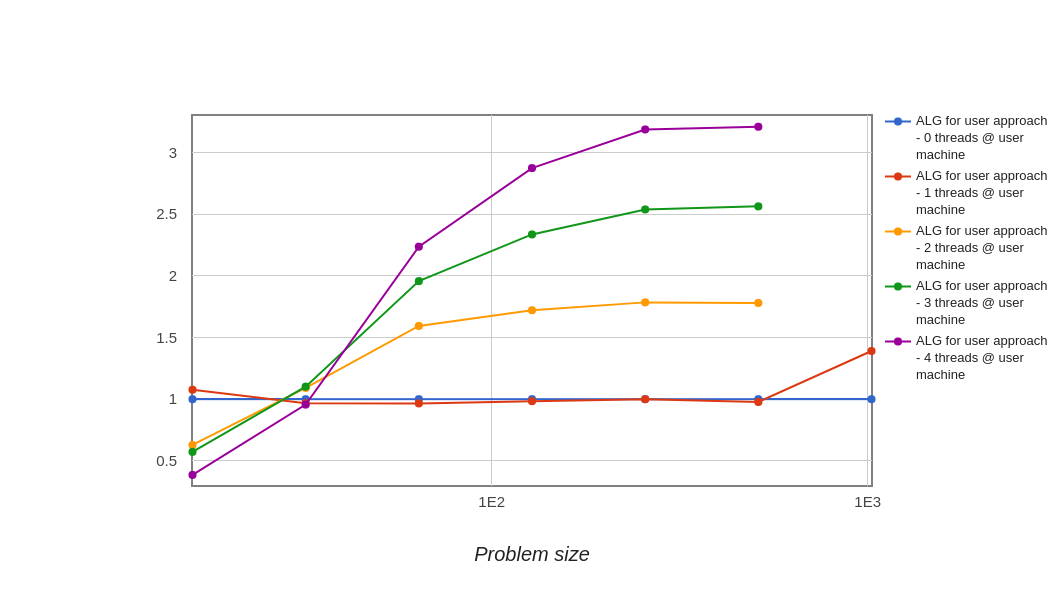
\includegraphics[width=\textwidth]{p2.png}
    \caption{Speedup vs problem size}
    \label{fig:p2}
\end{figure}
\begin{figure}[b]
    \centering
    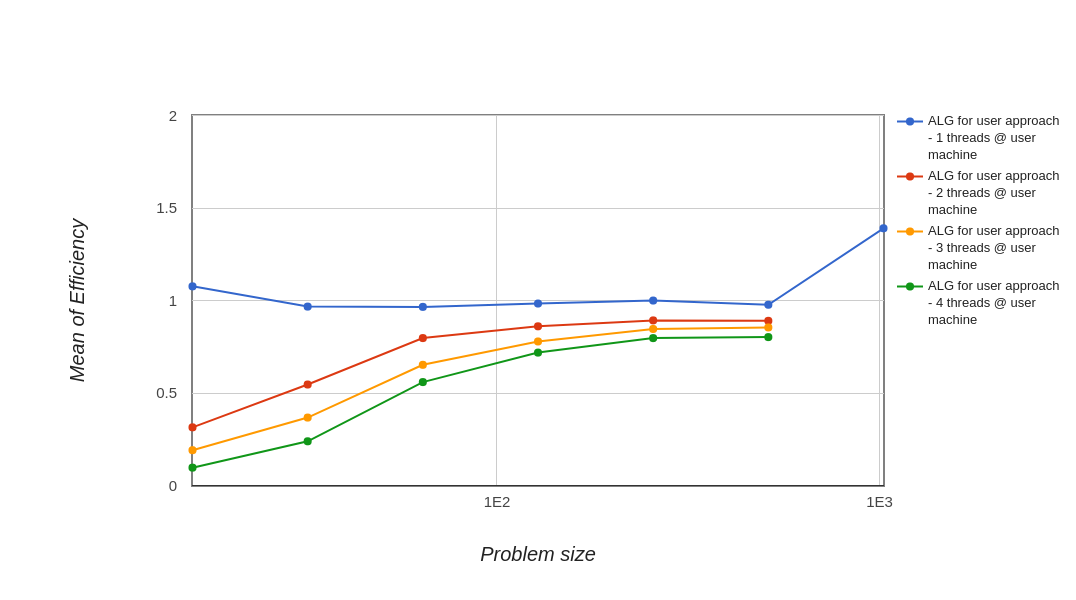
\includegraphics[width=\textwidth]{p3.png}
    \caption{Efficiency vs problem size}
    \label{fig:p3}
\end{figure}
\newpage

\section{Implementation Details(block matrix multiplication)}
\subsection{Brief and clear description about the Serial implementation}
This is a divide and conquer approach on traditional matrix multiplication. We recursively divide each matrix into smaller and smaller blocks, and perform multiplication and summation operations on them.
\subsection{Brief and clear description about the implementation of the approach (Parallelization Strategy, Mapping of computation to threads)}
Initially we distribute a different set of blocks to each thread. In the combine step of a level, the results of 2 threads are added into one matrix, and one thread hands over its entire data to another and dies. This step goes on until there is one thread surviving. This thread will hold the final result of the matrix multiplication.
\section{Complexity and Analysis}
\subsection{Complexity of serial code}
Cubic complexity $O(n^3)$
\subsection{Theoretical Speedup (using asymptotic analysis, etc.)}
n, where n is the total number of processors.
\section{Curve Based Analysis}
\subsection{Time Curve related analysis (as no. of processor increases)}
\begin{figure}[H]
    \centering
    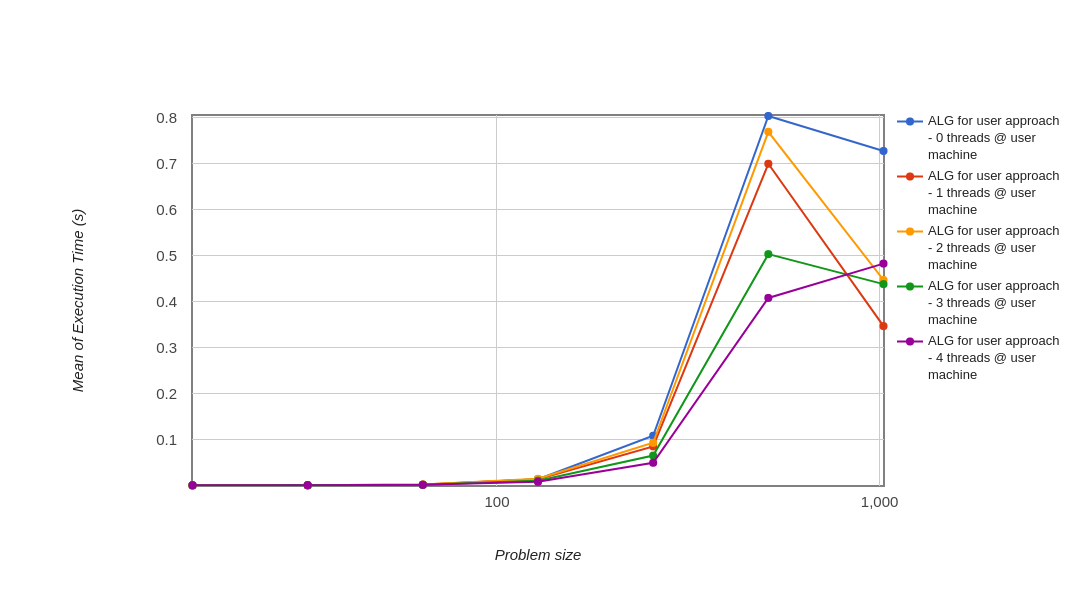
\includegraphics[width=\textwidth]{p4.png}
    \caption{Execution time for simple matrix multiplication}
    \label{fig:p4}
\end{figure}
For small problem sizes, the overhead of adding 1 extra core to the solution outweighs the advantages given by it. Thus for small input sizes, the execution time is higher for a higher number of cores. As the problem size increases, the overhead becomes insignificant in front of the compute time, which decreases drastically when a larger number of cores are used. This is quite natural because the work is shared equally amongst all processors.
\subsection{Speedup Curve related analysis (as problem size and no. of processors increase)}
The speedup is bound by "n", the number of cores. Therefore, irrespective of the problem size, the speedup is always lesser than n for n cores. For small problem sizes, the speedup is less than one if we use more cores. This again indicates that the load is too small to be parallelized efficiently. For very large problem sizes we see almost a constant speedup. This indicates that saturation has been achieved.  For 4 cores and a problem size of 512,  we get a speedup of approximately 2.09, whereas for 2 cores we get a speedup of 1.28.
\newpage
\begin{figure}[t]
    \centering
    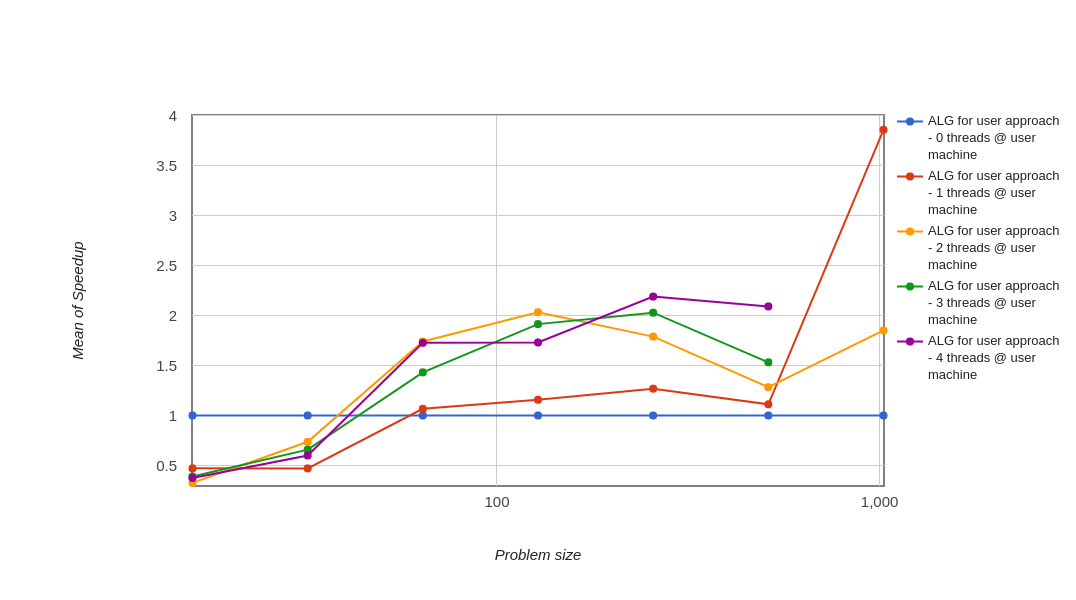
\includegraphics[width=\textwidth]{p5.png}
    \caption{Speedup vs problem size}
    \label{fig:p5}
\end{figure}
\begin{figure}[b]
    \centering
    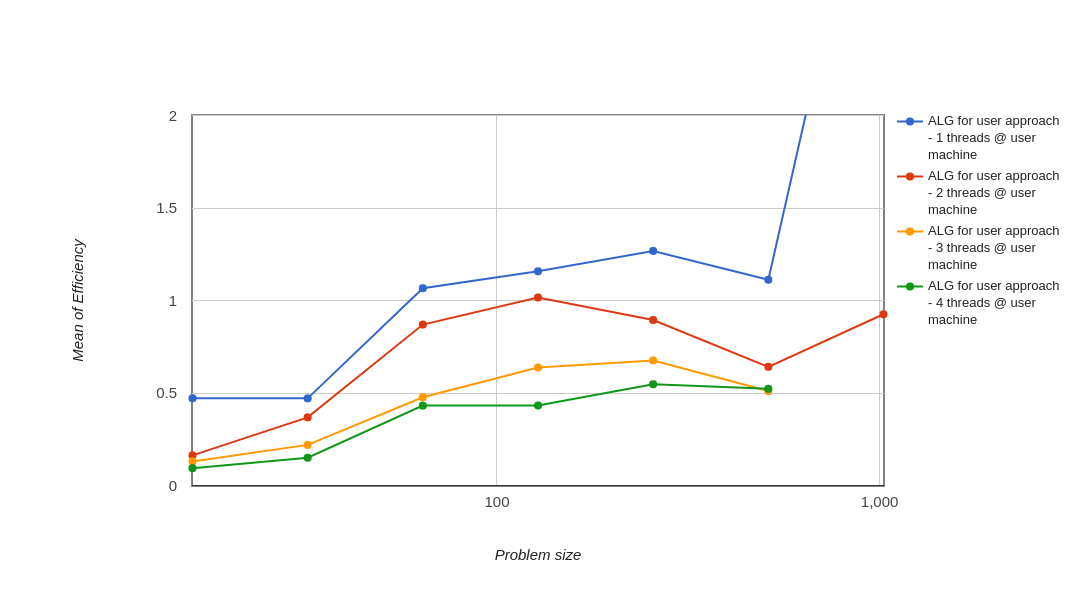
\includegraphics[width=\textwidth]{p6.png}
    \caption{Efficiency vs problem size}
    \label{fig:p6}
\end{figure}
\newpage
\end{document}

